
%%%%%%%%%%%%%%%%%%%%%%%%%%%%%%%%%%%%%%%%%%%%%%%%%%%%%%%%%%%%%%%%%%%%%
% LaTeX Template: Project Titlepage Modified (v 0.1) by rcx
%
% Original Source: http://www.howtotex.com
% Date: February 2014
% 
% This is a title page template which be used for articles & reports.
% 
% This is the modified version of the original Latex template from
% aforementioned website.
% 
%%%%%%%%%%%%%%%%%%%%%%%%%%%%%%%%%%%%%%%%%%%%%%%%%%%%%%%%%%%%%%%%%%%%%%

\documentclass[12pt]{article}
\usepackage[utf8]{inputenc}
\usepackage[a4paper]{geometry}
\usepackage[myheadings]{fullpage}
\usepackage{enumitem}
\usepackage{fancyhdr}
\usepackage{lastpage}
\usepackage{graphicx, wrapfig, subcaption, setspace, booktabs}
\usepackage[T1]{fontenc}
\usepackage[font=small, labelfont=bf]{caption}
\usepackage{fourier}
\usepackage{amsmath}
\usepackage[protrusion=true, expansion=true]{microtype}
\usepackage[english]{babel}
\usepackage{sectsty}
\usepackage{url, lipsum}
\usepackage{titlesec}
\usepackage{diagbox}
\usepackage{pdfpages}

\usepackage{listings}
\usepackage{color}

\definecolor{dkgreen}{rgb}{0,0.6,0}
\definecolor{gray}{rgb}{0.5,0.5,0.5}
\definecolor{mauve}{rgb}{0.58,0,0.82}

\lstset{frame=tb,
  language=C++,
  aboveskip=3mm,
  belowskip=3mm,
  showstringspaces=false,
  columns=flexible,
  basicstyle={\small\ttfamily},
  numbers=none,
  numberstyle=\tiny\color{gray},
  keywordstyle=\color{blue},
  commentstyle=\color{dkgreen},
  stringstyle=\color{mauve},
  breakatwhitespace=true,
  breaklines=true,
  tabsize=2
}

\newcommand{\HRule}[1]{\rule{\linewidth}{#1}}
\onehalfspacing
\setcounter{tocdepth}{5}
\setcounter{secnumdepth}{5}
\inputencoding{utf8}

\titleformat{\paragraph}
{\normalfont\normalsize\bfseries}{\theparagraph}{1em}{}
\titlespacing*{\paragraph}
{0pt}{3.25ex plus 1ex minus .2ex}{1.5ex plus .2ex}

%-------------------------------------------------------------------------------
% HEADER & FOOTER
%-------------------------------------------------------------------------------
\pagestyle{fancy}
\fancyhf{}
\setlength\headheight{15pt}
\fancyhead[L]{António Pedro Araújo Fraga}
\fancyhead[R]{Cranfield University}
\fancyfoot[R]{Page \thepage\ of \pageref{LastPage}}
%-------------------------------------------------------------------------------
% TITLE PAGE
%-------------------------------------------------------------------------------

\begin{document}

\title{ \fontsize{40}{90} \textsc{High Performance Computing}
		\\ [2.0cm]
		\HRule{0.5pt} \\
		\LARGE \textbf{Heat Conduction Equation}
		\HRule{2pt} \\ [0.5cm]
		\normalsize \today \vspace*{5\baselineskip}}

\date{}

\author{
		\textbf{António Pedro Araújo Fraga} \\
		\textbf{Student ID: 279654} \\ 
		\textbf{Cranfield University} \\
		\textbf{M.Sc. in Software Engineering for Technical Computing
		} }

\maketitle
\thispagestyle{empty}
\newpage
\tableofcontents
\thispagestyle{empty}
\newpage
\null\vspace{\fill}
\begin{abstract}
\normalsize
Three numerical schemes were applied to compute a solution for a parabolic partial differential equation, the heat conduction equation. It was used an explicit scheme and two implicit schemes. The solutions were computed both sequentially and in parallel making use of \textbf{MPI}, \textbf{M}essage \textbf{P}assing \textbf{I}nterface technology. Two pairs of \textbf{time} and \textbf{space} steps were studied, along with their effect on the solving system. \textbf{Speed-ups} of solutions computed with several processes were analysed, and their values were discussed. 

\end{abstract}
\vspace{\fill}
\thispagestyle{empty}
\newpage

%-------------------------------------------------------------------------------
% Section title formatting
\sectionfont{\scshape}
\titleformat{\section}
{\normalfont\huge\bfseries}{\thesection}{1em}{}
\titleformat{\subsection}
{\normalfont\large\bfseries}{\thesubsection}{1em}{}
\titlespacing*{\section}
{0pt}{5.5ex plus 1ex minus .2ex}{4.3ex plus .2ex}
\titlespacing*{\subsection}
{0pt}{5.5ex plus 1ex minus .2ex}{4.3ex plus .2ex}
%-------------------------------------------------------------------------------

%-------------------------------------------------------------------------------
% BODY
%-------------------------------------------------------------------------------

%-------------------------------------------------------------------------------
% Nomenclature
%-------------------------------------------------------------------------------
\begin{table}[tb]
\caption{Nomenclature}
\label{tab:notation}
\centering
\def\arraystretch{1.5}
\begin{tabular}{ll}
Diffusivity & $D$\\
First derivative in time & $\frac{\partial f}{\partial t}$\\
First derivative in space & $\frac{\partial f}{\partial x}$\\
Time grid position & $n$\\
Space grid position & $i$\\
Function at time and space grid position & $f_i^n$\\
Time step & $\Delta t$\\
Space step & $\Delta x$\\
Time value & $t$\\
Space value & $x$\\
Analytical function at specific space and time values& $f(x, t)$\\
Initial Temperature& $T_{in}$\\
Surface Temperature& $T_{sur}$\\
\end{tabular}
\end{table}

%-------------------------------------------------------------------------------
% Introduction
%-------------------------------------------------------------------------------

\section*{Introduction}
\addcontentsline{toc}{section}{Introduction}

Numerical methods are used to obtain an approximated solution for a given problem. The exact solution of those problems are usually computed in \textbf{Nondeterministic Polynomial Time}, therefore an approximated solution is often accepted. The approximation factor is often related with the number of space steps that a time step is split on. A high number of space steps leads to a more accurate solution, keeping in mind the existence of \textbf{round-off} errors \cite{fraga}.

\par Although, decreasing the value of space steps results in a more "computational hungry" process. Which means that the time used to compute a solution increases, unless several processes are used to compute the final solution. Parallel computing is simple if it's done with \textbf{independent} data. In this case, there's no need to exchange data between workers. Sometimes the methods used to compute the solution have dependencies between space steps calculations. Thus, unless a process communicates with different processes, it's not possible to compute an approximated solution. 

\par The challenge is to minimize the communication overhead. To achieve that, one has to keep in mind how to perform communications. Deciding \textbf{when} and \textbf{how} to \textbf{exchange} data between processes.

\par Memory management plays an important role on \textbf{efficiency} as well. A program is split into \textbf{segments}, and each segment is split into \textbf{pages}. The size of each segment depends of the compiler. Each of them contains important data like the \textbf{stack}, \textbf{heap}, and actual data. But each \textbf{page} is divided into equal parts, \textbf{4kb} on UNIX based systems. Therefore, whenever a program accesses an address, a page is loaded into \textbf{cache}, which is a very fast type of memory close to the \textbf{CPU}. This means that accessing memory within the same page won't add the overhead of moving the data from the main memory to cache again. Such knowledge might make one think of how to write specific parts of the code.  

\subsection*{Problem definition}
\addcontentsline{toc}{subsection}{Problem definition}

The problem is defined in the previously developed \textbf{report}\cite{fraga} for \textbf{Computational Methods} \& \textbf{C++} modules. It is intended to examine the application of distributed memory parallel programming techniques on the referred problem.

\subsection*{Analysis}
\addcontentsline{toc}{subsection}{Analysis}
\par The analysis of \textbf{parallel programming} can be done by measuring times of execution. One should measure the time of execution with a single process, comparing it with the execution time in parallel with \textbf{p} processors. Therefore, the \textbf{Speedup} concept can be defined\cite{speedup},
\newline
\begin{center}
$
	Speedup(P) = \frac{Time_{Sequential}}{Time_{parallel}(P)}
$
\end{center}
\hfill
\par It is important to define the concept of \textbf{Theoretical Speedup} as well. Whenever a program is computed in parallel, the optimal speedup is obtained by taking the number of processes used to compute a solution. Often, the \textbf{Optimal Speedup} is difficult to be achieved. This happens because the solution is computed in a distributed system. Processes, by default, are not able to access data from different processes easily. One must use a form of \textbf{IPC}, or \textbf{I}nter \textbf{P}rocess \textbf{C}ommunication. The \textbf{MPI} technology offers an \textbf{API} to achieve that. 

\section*{Procedures}
\addcontentsline{toc}{section}{Procedures}

\par Every solution was computed on \textbf{Delta}, a supercomputer located at Cranfield University. The computational time was measured by using the \textbf{MPI Wtime} call, and assuring that every process was entering and leaving the computation of a given method at the same time. 
\par Three different schemes/methods were used to compute a solution for the given problem, sequentially and in parallel. One of them is an explicit schemes, \textbf{Forward in Time, Central in Space}, and two of them are implicit schemes, \textbf{Laasonen Simple Implicit} and \textbf{Crank-Nicholson}. Two pairs \textbf{space} and \textbf{time} steps were studied,
\begin{itemize}[noitemsep] 
\item $ \Delta t = 0.1 $ and $ \Delta x = 0.5$
\item $ \Delta t = 0.001 $ and $ \Delta x = 0.005$
\end{itemize}
It was seen in the previous work\cite{fraga} that these schemes can be written in its discretized form.

\par A \textbf{time step} can be defined as an array, divided by the number of space steps to be computed. In a sequential algorithm, the process handles the entire domain. Since it was intended to parallelize the computational method, the \textbf{time step} can be divided into \textbf{p} \textbf{almost equal} parts, with \textbf{p} being the number of processes available. Notice that having \textbf{more} processes than space steps is an exception. Thereby, the \textbf{lower} and \textbf{upper} bounds of space steps to be computed by a process can be determined by it's ranking.
\newline
\begin{center}
\large
\begin{minipage}{.5\textwidth}
  \centering
  $
  	lower = \frac{ranking \times number_{Space Steps} }{number_{Processes}}
  $
\end{minipage}%
\begin{minipage}{.5\textwidth}
  \centering
  $
  	upper = \frac{ (ranking + 1) \times number_{Space Steps} }{number_{Processes}} - 1
  $
\end{minipage}
\end{center}
\hfill
\par Defining these values as integers will avoid any kind of \textbf{floating point} values.
\par We can not, however, define these rules if it happens to have more available processes than space steps. In this case, only the number of processes corresponding to the number of space steps can be used.
\par Notice that the process with the $\textbf{rank} = 0$, computes the first window of values, whereas the process with $\textbf{rank} = 1$ computes the second window of values. The same idea is replicated to the next processes and windows.

\subsection*{Explicit Scheme}
\addcontentsline{toc}{subsection}{Explicit Scheme}

\par It is known that these type of schemes rely only on values from the previous time steps to compute the solution\cite{fraga}. Therefore, once one has access to this values, it is possible to compute the values for the current time step. In this cases, processes that need values from different workers, can obtain them by using the MPI API.

\subsubsection*{Forward in Time Central in Space}
\addcontentsline{toc}{subsubsection}{Forward in Time Central in Space}

\par The stencil for this scheme can be observed on \textbf{Figure 1}. When computing the \textbf{first} time step for this scheme, the previous time step values correspond to the \textbf{initial conditions}. This means that no data had to be exchanged during the calculations of that iteration. Every process had knowledge of these conditions.

\begin{figure}[!htb]
  \centering
  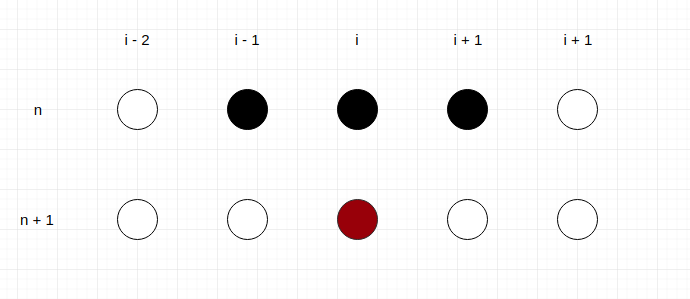
\includegraphics[width=.6\linewidth]{FTCS.png}
  \captionof{figure}{Forward in Time Central in Space method stencil.}
\end{figure}

\par However, the next time steps calculations of each process required values that didn't exist in their memory. \textbf{Non-blocking} communication was used to exchange dependable data. It was known that the next iteration to be computed by those processes needed the first time step value from the processes that were responsible to compute the next window of values. Therefore, whenever a process finished to compute the first value of an iteration, was responsible to send that value to the previous process. With the exception of the \textbf{root} process, that knows the value from the \textbf{Initial Conditions}. By this time, the processes could expect to receive a value from the next process, so the same \textbf{Non-blocking} communication was used to obtain it. \textbf{Figure 2} contains a graphic representation of the sending messages on the first iteration.
\newline
\begin{figure}[!htb]
  \centering
  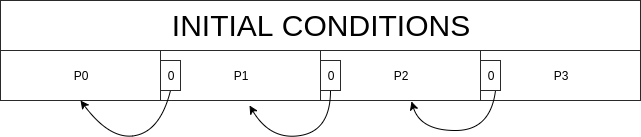
\includegraphics[width=.7\linewidth]{fcts_comm1.png}
  \captionof{figure}{Processes sending first value to the previous worker.}
\end{figure}
\hfill
\par Following the same mindset, whenever a process reached the last value to be computed, it was sending that information to the process responsible for the next window. Knowing that it would have to receive a value from the previous process. Notice that the \textbf{ranking} of the receiving process could be discovered by incrementing its own ranking, and the ranking of the sending process was found by decrementing it. The process with the highest ranking was not sending or receiving any value from the next worker, because there was none. It could also access to the surface temperature value, a \textbf{known} and constant variable. The graphical representation of this phase can be observed on \textbf{Figure 3}.
\newline
\begin{figure}[!htb]
  \centering
  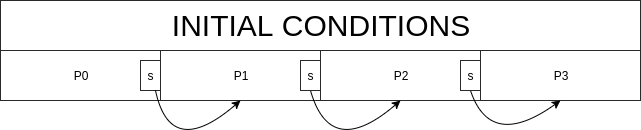
\includegraphics[width=.7\linewidth]{fcts_comm2.png}
  \captionof{figure}{Processes sending first value to the previous worker.}
\end{figure}
\hfill

\par The advantage of using \textbf{Non-blocking} communication, is that processes didn't have to go into the \textbf{waiting} state whenever they were sending or receiving messages. The \textbf{MPI Wait} call was used by the time processes were about to use those values. For the next iteration, whenever a process was computing the first and last value of its own window, it had to wait for the receiving value. The process would enter into a \textbf{waiting} state if the request was not fulfilled by that time. 

\par This mechanism of communication was used in nearly every time step calculations, \textbf{except} for the \textbf{first} and \textbf{last} one, when there was no need of communications.

\subsection*{Implicit Schemes}
\addcontentsline{toc}{subsection}{Implicit Schemes}

\par Implicit schemes rely on both previous and current time step in order to calculate the desired value\cite{fraga}. The methods stencil can be observed on \textbf{Figure 4} and \textbf{Figure 5}. 

\begin{figure}[!htb]
\centering
\begin{minipage}{.5\textwidth}
  \centering
  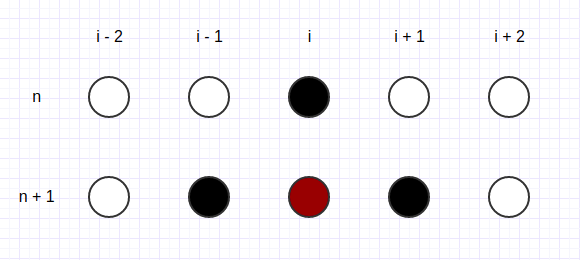
\includegraphics[width=.8\linewidth]{laasonen.png}
  \captionof{figure}{Laasonen's method stencil.}
\end{minipage}%
\begin{minipage}{.5\textwidth}
  \centering
  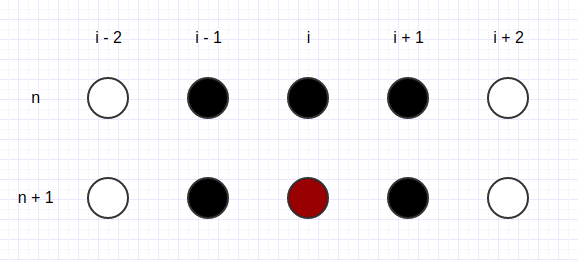
\includegraphics[width=.8\linewidth]{crank-nicholson.png}
  \captionof{figure}{Crank-Nicholson's method stencil.}
\end{minipage}
\end{figure}

The time step computation of these schemes requires that a special form of a linear system of equations to be solved. This system $Ex = b$ contains a \textbf{tridiagonal matrix}, the matrix \textbf{E}, which can be divided into two different matrices, \textbf{A} and \textbf{S}\cite{spike}. In case of a sequential code, the \textbf{Thomas Algorithm} is the most efficient solution. With a parallel code, the \textbf{spike} algorithm can be used to solve dependencies among processes. The results can be achieved by splitting the computation methodology into three different phases.

\begin{itemize}[noitemsep] 
\item Solve $\textbf{Ay = b}$ in parallel.
\item Gather the top and bottom values of \textbf{y} into one process and solve dependencies, computing a vector \textbf{x}. Broadcast the solution.
\item Solve $\textbf{Sx = y}$ in parallel.
\end{itemize}

\par Since the matrix \textbf{A} is a \textbf{tridiagonal} matrix, it can be divided into several smaller matrices, a \textbf{block tridiagonal matrix}\cite{chang}, like seen in \textbf{Figure 6}. Each process was responsible to solve a smaller linear system of equations, obtaining its own \textbf{y} array.
\newline
\begin{figure}[!htb]
  \centering
  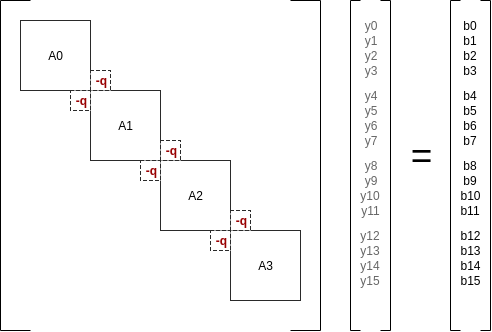
\includegraphics[width=.55\linewidth]{spikedivision.png}
  \captionof{figure}{Division of main matrix in blocks.}
\end{figure}


\par This implies that several variables are not used in this phase (\textbf{-q}). Thus, two different arrays were created\cite{spike}, \textbf{v'} and \textbf{w'},
\newline
\begin{center}
\begin{minipage}{.5\textwidth}
  \centering
 $
v' = 
\begin{bmatrix}
	0 \\
	0 \\
    \dots \\
    -q \\
\end{bmatrix}
$
\end{minipage}%
\begin{minipage}{.5\textwidth}
  \centering
   $
w' = 
\begin{bmatrix}
	-q \\
	\dots \\
    0 \\
    0 \\
\end{bmatrix}
$
\end{minipage}
\end{center}

\par These arrays were used to compute the \textbf{spikes} arrays. They can be computed by solving $\textbf{Av = v'}$ and $\textbf{Aw = w'}$, creating two different arrays, \textbf{v} and \textbf{w}. And since \textbf{A} is a tridiagonal matrix, they can be computed with \textbf{Thomas Algorithm} as well. These arrays are useful to create the matrix \textbf{S} of the last phase of the \textbf{spike} algorithm. 

\par In order to solve the $\textbf{Sx = y}$, one has to solve a special form of this equation first. Involving every \textbf{top} and \textbf{bottom} element of the \textbf{y} array of each process, forming the array $\textbf{y'}$. This information was gathered by the \textbf{root} process. In order to solve dependencies between processes, the $\textbf{S'x' = y'}$ system was solved. Note that the $v_t$,  $v_b$, $w_t$ and $w_b$ values are the \textbf{top} and \textbf{bottom} values of both \textbf{v} and \textbf{w} arrays, the \textbf{spike arrays}, that were previously calculated.
\newline
\begin{center}
$
\begin{bmatrix}
    1 & 0 & v_t &  &  &  &  & \\
    0 & 1 & v_b &  &  &  &  &  \\
     & w_t & 1 & 0 & v_t &  &  &  \\
   	 & w_b & 0 & 1 & v_b &  &  & \\ 
   	 &  &  & w_t & 1 & 0 & v_t &  \\
   	 &  &  & w_b & 0 & 1 & v_b &  \\
   	 &  &  &  &  & w_t & 1 & 0 \\
   	 &  &  &  &  & w_b & 0 & 1 \\
\end{bmatrix}
\begin{bmatrix}
    x'0_t \\
    x'0_b \\
    x'1_t \\
    x'1_b \\
    x'2_t \\
    x'2_b \\
    x'3_t \\
    x'3_b \\
\end{bmatrix}
=
\begin{bmatrix}
    y'0_t \\
    y'0_b \\
    y'1_t \\
    y'1_b \\
    y'2_t \\
    y'2_b \\
    y'3_t \\
    y'3_b \\
\end{bmatrix}
$
\end{center}

\par This system of equations can be solved by using the \textbf{Gaussian Elimination} method, and the $\textbf{x'}$, can be \textit{broadcasted} to the rest of the processes. 
\par The last phase consists of solving the $\textbf{Sx = y}$ system, that can be defined in  \textbf{Figure 7}.

\begin{figure}[!htb]
  \centering
  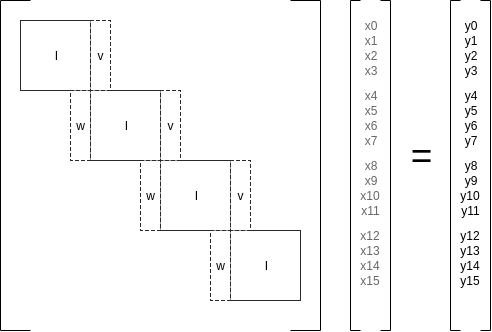
\includegraphics[width=.55\linewidth]{Sxy.png}
  \captionof{figure}{Sx = y system of equations.}
\end{figure}

\par Therefore, the solution can be obtained with\cite{spike},

\[
\left\{ 
\begin{array}{c}
X_0 = Y_0 - V X_1^t \\ 
X_{j} = Y_{j} - V X_{j + 1}^t - W X_{j - 1}^b \\ 
X_{P - 1} = Y_{P - 1} - W X_{P - 2}^b
\end{array}
\right. 
\]

\section*{Results \& Discussion}
\addcontentsline{toc}{section}{Results \& Discussion}

\par In this section the results of the experiments were analysed. Starting by observing \textbf{Figure 8}, it can be seen that the solution of the \textbf{explicit} scheme is not accurate at these conditions. Notice that this solution was computed by \textbf{4} processes, with a $ \Delta t = 0.001 $ and $ \Delta x = 0.005$. This phenomenon can be explained by making the stability analysis of this method\cite{fraga}. On this conditions, this method is unstable, therefore it can not present an approximated solution. It can be seen that the implicit schemes, however, were able to present good results.

\begin{figure}[!htb]
\centering
\begin{minipage}{.28\textwidth}
  \centering
  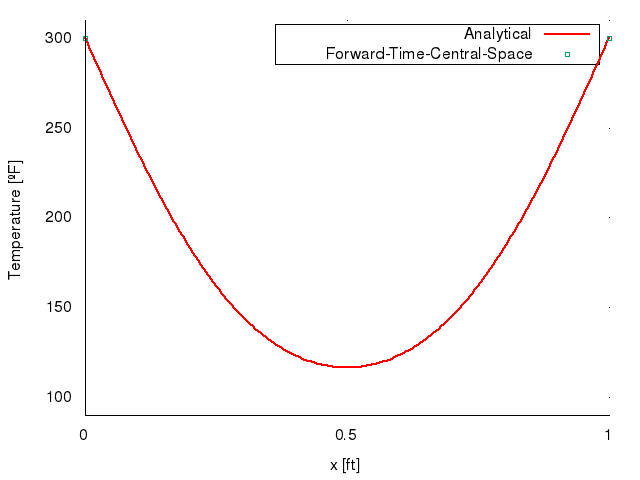
\includegraphics[width=1\linewidth]{ftcs.png}
\end{minipage}%
\begin{minipage}{.28\textwidth}
  \centering
  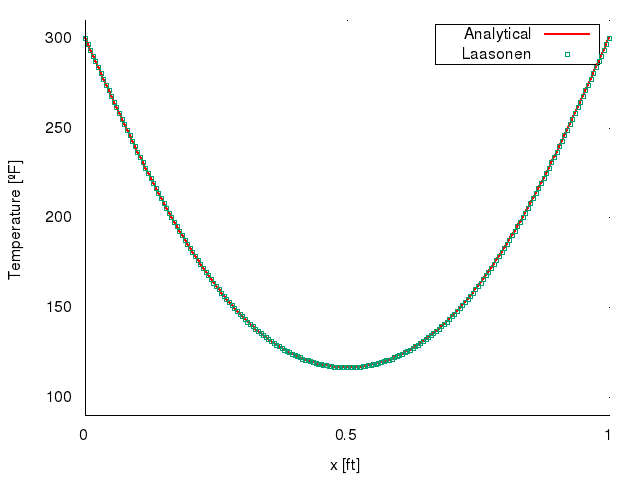
\includegraphics[width=1\linewidth]{laa.png}
\end{minipage} %
\begin{minipage}{.28\textwidth}
  \centering
  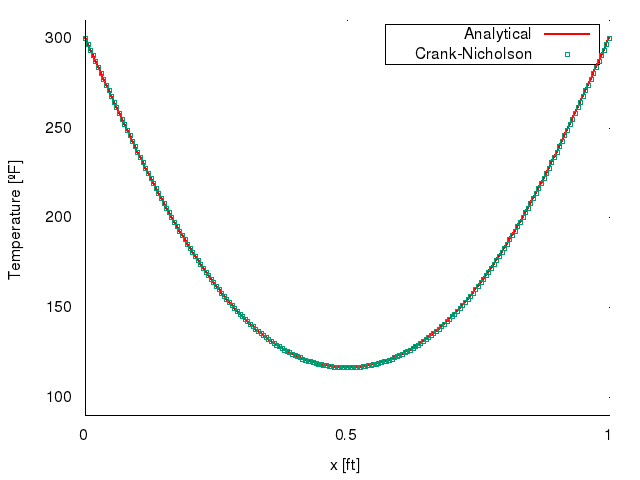
\includegraphics[width=1\linewidth]{cn.png}
\end{minipage}
\captionof{figure}{FTCS, Laasonen and Crank-Nicholson solutions calculated with 4 processors, at t = 0.4, with $ \Delta t = 0.001 $ and $ \Delta x = 0.005$.}
\end{figure}

\par As referred, it was possible to measure the computation time of a given method. The results for a sequential calculations were quite similar to the previous results\cite{fraga}. The execution time of a solution for \textbf{$ \Delta t = 0.001 $ and $ \Delta x = 0.005$} did was stable as the number of processes were increased. This happened because the \textbf{software} implementation allowed only one process to work. Notice that under these conditions, each time step contains \textbf{three} different values. \textbf{Two} of those values are known, as they are considered as \textbf{initial conditions}. Therefore, there was only one value to be computed for every time step. 

\par The results of a parallel execution for the \textbf{$ \Delta t = 0.001 $ and $ \Delta x = 0.005$} can be observed on \textbf{Figure 9}. Under these conditions, \textbf{199} values had to be computed for every time step. By observing the figure, and comparing the sequential solution execution time of the methods, we can see a continuous improvement of the \textbf{Forward in Time, Central in Space} scheme. This improvement couldn't be replicated by the implicit schemes. The execution time of these schemes started to increase when the solution was calculated by more than \textbf{four} processes. 

\par It was referred that the dependencies among the several processes computing the \textbf{Forward in Time, Central in Space} solution were handled using \textbf{non-blocking} communication. Whereas the implicit schemes were using a blocking communication to solve their dependencies. A blocking communication was used because the \textbf{second} phase of the \textbf{spike} algorithm required a sequential flow of data. Thereby, one can conclude that this phase was a major bottleneck while measuring the execution time of these solutions. 

\begin{figure}[!htb]
\centering
\begin{minipage}{.5\textwidth}
  \centering
  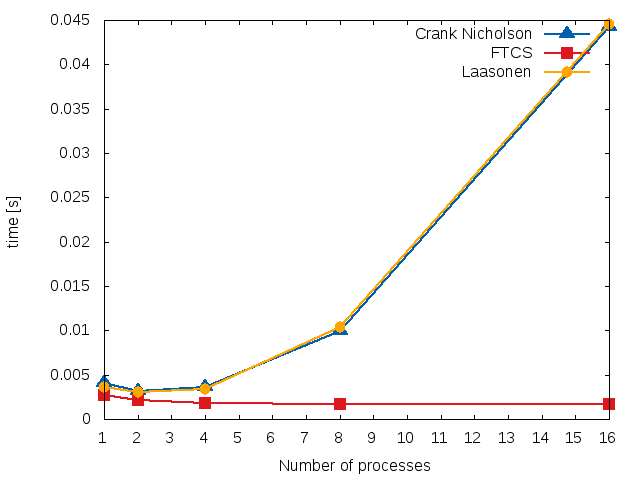
\includegraphics[width=1.0\linewidth]{times.png}
  \captionof{figure}{Comparison of execution times.}
\end{minipage}%
\begin{minipage}{.5\textwidth}
  \centering
  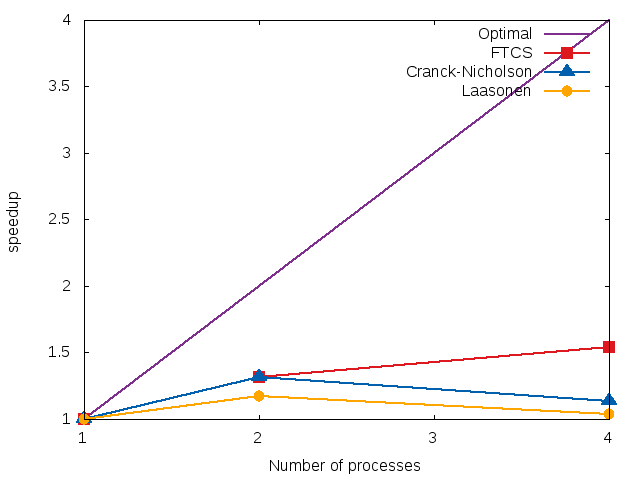
\includegraphics[width=1.0\linewidth]{speedup.png}
  \captionof{figure}{Speedup of each method.}
\end{minipage}
\end{figure}

\par However, while observing \textbf{Figure 10}, it could be seen that the \textbf{speedup} value of the \textbf{Forward in Time, Central in Space} scheme is far from its optimal value. In fact this value is significantly low. A larger \textbf{speedup} value would be seen while computing a larger grid. In such small system, the bottleneck of communications is high, and therefore one can not obtain big improvements. An experiment with a system of \textbf{thousands} of elements in each time step would contribute to a higher \textbf{speedup}.

\pagebreak
\section*{Conclusions}
\addcontentsline{toc}{section}{Conclusions}

\par The obtained results could support the theoretical concepts. Unstable methods demonstrated an error growth through the time progress. The \textbf{Forward in Time, Central in Space} explicit scheme was stable with the given initial conditions, therefore it could support a good solution for the explicit stable scheme, \textbf{DuFort-Frankel}. As referred, the solution of the DuFort-Frankel method strongly depends on the first iteration solution.
\par It could be observed that smaller steps can lead to a time expensive solution, whereas larger steps lead to an error increase. Stable methods could give a good solution with the right time and space steps, but by analysing the second norm value, it was concluded that the Crank-Nicholson method is more accurate. This is due to the fact that this method has a better approximation order.
\par It is important to have a balance between the two problems (time and approximation), a method should be computed in an acceptable time, and still obtain a good result. In realistic scenarios the problem solution is not known, therefore error estimates are impractical. The used step size should be small as possible, as long as the solution is not dominated with round-off errors. The solution must be obtained with a number of steps that one has time to compute. 
 

%-------------------------------------------------------------------------------
% REFERENCES
%-------------------------------------------------------------------------------
\newpage
%\addcontentsline{toc}{section}{References}
\begin{thebibliography}{0}

\bibitem{fraga}
António Pedro Fraga, December 2017, \textit{Heat Conduction Equation, C++ \& Computational Methods}, Available at: <\url{http://pedrofraga.me/heat-conduction-equation.pdf}> [Accessed 24 January 2018]

\bibitem{speedup}
Multiple authors, May 2017, \textit{A Comprehensive Linear Speedup Analysis for Asynchronous Stochastic Parallel Optimization from Zeroth-Order to First-Order}, Available at: <\url{http://xrlian.com/res/Asyn_Comprehensive/paper.pdf}> [Accessed 24 January 2018]

\bibitem{chang}
Li-Wen Chang, 2014, \textit{Scalable Parallel Tridiagonal Algorithms with Diagonal Pivoting and their optimization for Many-Core Architectures}, Available at: <\url{http://impact.crhc.illinois.edu/shared/Papers/Chang-Thesis-2014.pdf}> [Accessed 25 January 2018]

\bibitem{spike}
Eric Polizzi, Ahmed H. Sameh, February 2016, \textit{A parallel hybrid banded system solver: the SPIKE algorithm}, Available at: <\url{http://impact.crhc.illinois.edu/shared/Papers/Chang-Thesis-2014.pdf}> [Accessed 25 January 2018]


\end{thebibliography}
\newpage

\section*{Appendices}
\addcontentsline{toc}{section}{Appendices}



\end{document}

